\documentclass[border=8pt]{standalone}
\usepackage{tikz}
\usetikzlibrary{arrows.meta,positioning,calc}
\begin{document}
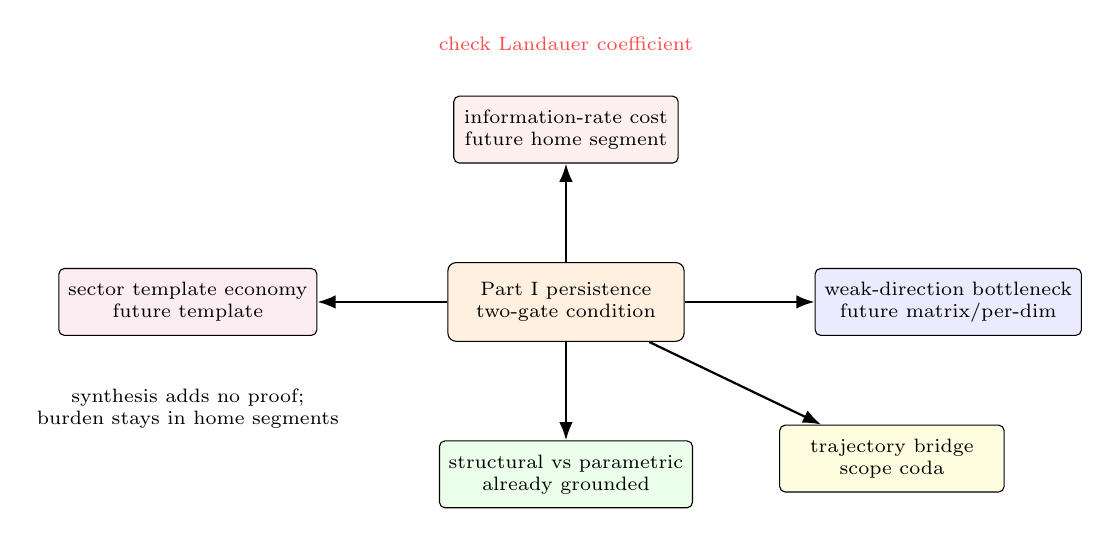
\begin{tikzpicture}[
  hub/.style={draw, rounded corners=3pt, align=center, minimum width=3.0cm, minimum height=1.0cm, font=\scriptsize, fill=orange!12},
  box/.style={draw, rounded corners=2pt, align=center, minimum width=2.85cm, minimum height=0.85cm, font=\scriptsize},
  note/.style={align=center, font=\scriptsize},
  arr/.style={-Latex, thick}
]

\node[hub] (p) {Part I persistence\\two-gate condition};
\node[box, fill=red!6, above=1.25cm of p] (cost) {information-rate cost\\future home segment};
\node[box, fill=blue!8, right=1.65cm of p] (weak) {weak-direction bottleneck\\future matrix/per-dim};
\node[box, fill=green!8, below=1.25cm of p] (struct) {structural vs parametric\\already grounded};
\node[box, fill=purple!7, left=1.65cm of p] (template) {sector template economy\\future template};
\node[box, fill=yellow!12, below right=1.05cm and 1.2cm of p] (identity) {trajectory bridge\\scope coda};

\draw[arr] (p) -- (cost);
\draw[arr] (p) -- (weak);
\draw[arr] (p) -- (struct);
\draw[arr] (p) -- (template);
\draw[arr] (p) -- (identity);

\node[note, above=0.45cm of cost, text=red!70] {check Landauer coefficient};
\node[note, below=0.55cm of template] {synthesis adds no proof;\\burden stays in home segments};

\end{tikzpicture}
\end{document}
